%% IEEE Conference Paper — HAN++: Patient-Conditioned Hierarchical Attention for Multi-Label Disease Prediction
%% HAN++ Project — Group 17, University of Moratuwa
%% Ethics Approval: EDN/2026/004
%% Compile: pdflatex main.tex && bibtex main && pdflatex main.tex && pdflatex main.tex

\documentclass[conference]{IEEEtran}
\IEEEoverridecommandlockouts

% ── Packages ──────────────────────────────────────────────────────────────────
\usepackage{cite}
\usepackage{amsmath,amssymb,amsfonts}
% Note: algorithmic removed to avoid conflict with algpseudocode/algorithmicx
\usepackage{graphicx}
\usepackage{textcomp}
\usepackage[table]{xcolor}
\usepackage{booktabs}
\usepackage{multirow}
\usepackage{array}
\usepackage{url}
\usepackage{hyperref}
\usepackage{subcaption}
\usepackage{algorithm}
\usepackage{algpseudocode}
\usepackage{bm}
\usepackage{amsthm}

\newtheorem{definition}{Definition}
\newtheorem{proposition}{Proposition}
\newtheorem{remark}{Remark}

\hypersetup{
  colorlinks=true,
  linkcolor=blue!60!black,
  citecolor=blue!60!black,
  urlcolor=blue!60!black,
  bookmarks=true
}

% ── Title ─────────────────────────────────────────────────────────────────────
\title{HAN++: Patient-Conditioned Hierarchical Attention\\for Multi-Label Disease Prediction from Heterogeneous EHR Graphs}

\author{
  \IEEEauthorblockN{Anushka Samaranayake,\quad
                    JohnPeter Charles,\quad
                    Tashin Kavishan,\quad
                    Mailki Meghana Wickramasinghe}
  \IEEEauthorblockA{Department of Electronic and Telecommunication Engineering /
                    Biomedical Engineering,\\
                    University of Moratuwa, Sri Lanka\\
                    \{anushkasandeepa522, jpcharlie02,
                      tashinkavishan123, malkimeghana1\}@gmail.com}
}

\begin{document}

\maketitle

% ── Abstract ──────────────────────────────────────────────────────────────────
\begin{abstract}
Predicting disease risk from Electronic Health Records (EHRs) requires
models that output calibrated probability scores --- not mere binary
flags --- together with uncertainty estimates for safe clinical deployment.
This paper presents \textbf{HAN++}, an improved Hierarchical Attention
Network that constructs a heterogeneous medical graph with four node
types (Patient, Symptom/Test, Organ, Disease) and derives meta-path-based
patient similarity relations via adjacency matrix composition
(e.g., $\mathbf{M}^{\text{PDP}} = \mathbf{A}_{PD}\mathbf{A}_{PD}^{\top}$).
HAN++ introduces three extensions over the original HAN:
(i)~multi-head ($M{=}4$) node-level attention per meta-path,
(ii)~\textbf{patient-conditioned semantic attention} --- a novel mechanism
that replaces HAN's global query vector with a patient-specific query
$\mathbf{q}_i = \mathbf{W}_q \mathbf{h}_i$, enabling each patient to
weight meta-paths according to their own clinical profile, and
(iii)~Monte Carlo Dropout uncertainty quantification providing
per-disease confidence intervals.
For each of the 9 tracked disease categories, the model outputs a
continuous probability score $\hat{p}_{i,d} \in [0,1]$ and an
uncertainty estimate $\sigma_{i,d}$; a disease-specific Youden-optimal
threshold $\theta_d$ converts scores to clinical decisions when needed.
Two-level attention interpretability (semantic $\boldsymbol{\beta}$
and node-level $\boldsymbol{\alpha}$) enables physician-facing
explanations of each prediction.
On an ethics-approved EHR dataset (EDN/2026/004) from CareCode (PVT)~Ltd
covering six Sri Lankan hospitals (48,546 patients, 107 clinical tests,
9 disease categories), HAN++ achieves
\textbf{F1-Macro = 0.9378}, \textbf{AUC-ROC = 0.9992}, and
\textbf{Brier score = 0.0192} (reduced to 0.0040 via temperature scaling).
While GridSearch-tuned traditional baselines achieve competitive F1-Macro
on this high-confidence dataset (Decision Tree: 0.9458), HAN++ provides
three critical clinical advantages they cannot: (1)~per-prediction
uncertainty quantification via MC Dropout ($3.7\times$ error enrichment
at the deferral threshold), (2)~patient-conditioned attention
interpretability showing \emph{which} clinical relationships drove each
prediction, and (3)~calibrated probability outputs suitable for
risk-stratified decision-making.
Unseen patient validation ($n{=}20$) achieves Mean AUC = 0.8934.
Multi-seed stability confirms $\text{F1-Macro} = 0.9397 \pm 0.0013$.
Attention faithfulness tests show removing the dominant meta-path
(P-D-P) collapses F1-Macro from 0.9378 to 0.4176, confirming
attention weights genuinely drive predictions.
\end{abstract}

\begin{IEEEkeywords}
Electronic Health Records, Hierarchical Attention Network, Graph Neural
Networks, Heterogeneous Graphs, Multi-organ Disease Prediction, Meta-path,
Patient-Conditioned Attention, MC Dropout, Uncertainty Quantification,
Attention Interpretability, Clinical Decision Support, Heterogeneous Graph
\end{IEEEkeywords}

% ── Section 1: Introduction ───────────────────────────────────────────────────
\section{Introduction}
\label{sec:intro}

Electronic Health Records (EHRs) contain rich longitudinal clinical
information --- laboratory test results, demographic data, and disease
histories --- that, when analysed effectively, can enable early
identification of multi-organ deterioration and support timely clinical
intervention \cite{obermeyer_2016, rajpurkar_2022}.
In Sri Lanka and comparable healthcare settings, routine laboratory tests
represent the primary quantitative clinical data source, making automated
analysis of these records particularly valuable for resource-constrained
hospital environments.

\subsection{Why Graph-Based Clinical Reasoning?}
\label{subsec:motivation}

Clinical test results are not independent features --- a patient's creatinine,
BUN, and eGFR collectively signal renal dysfunction far more than any individual
value.
Flat classifiers (DT, RF, XGBoost) treat each patient as an isolated feature
vector, discarding the relational structure that clinicians routinely exploit:
comorbidity co-occurrence, organ-system correlations, and population-level
patient similarity.
On our high-confidence dataset where disease labels are derived from
test-value thresholds, flat classifiers achieve strong F1-Macro (DT: 0.9458)
by learning the underlying threshold rules --- but they provide no uncertainty
quantification, no patient-conditioned interpretability, and no calibrated
probability outputs.
These three capabilities are essential for clinical deployment
(Sections~\ref{subsec:deferral}--\ref{subsec:faithfulness}).
The GNN literature confirms broader advantages of relational reasoning:
Sun et al.\ \cite{sun_2021} show 12--18\% improvements using
patient--disease graphs, and Oss Boll et al.\ \cite{oss_boll_2024}
survey 41 studies showing GNN benefits on EHR tasks.

\subsection{Model Development and Evolution}
\label{subsec:evolution_intro}

HAN++ was developed through a principled progression of graph neural
architectures.
In the feasibility phase, SeHGNN \cite{yang_2023} was evaluated as an
efficient heterogeneous GNN baseline (F1-Macro $\approx 0.63$).
At mid-review, a standalone pyHGT model \cite{hu_2020} was the strongest
available GNN architecture (F1-Macro = 0.7550).
HAN++ was developed to address pyHGT's key limitation --- the absence of
clinically-motivated meta-path hierarchy --- and achieves
F1-Macro = 0.9378 with AUC-ROC = 0.9992 on the final high-confidence
dataset (48,546 patients, 9 diseases).

\subsection{Contributions}
\label{subsec:contributions}

\begin{enumerate}
  \item \textbf{Clinical decision support system}: an end-to-end pipeline
        integrating EHR data ingestion, heterogeneous graph construction,
        HAN++ inference, and a two-phase disease risk scoring and test
        recommendation workflow (Fig.~\ref{fig:workflow}).
  \item \textbf{HAN++}: an improved Hierarchical Attention Network with
        four-head node-level attention per meta-path, achieving
        F1-Macro = 0.9378, F1-Micro = 0.9874, AUC-ROC = 0.9992.
  \item \textbf{Patient-Conditioned Semantic Attention} (\textit{novel}):
        we replace HAN's global query vector with a patient-specific query
        $\mathbf{q}_i = \mathbf{W}_q \mathbf{h}_i$, enabling per-patient
        meta-path weighting ($\boldsymbol{\beta} \in \mathbb{R}^{N \times K}$
        instead of $\mathbb{R}^K$).
        To our knowledge, no prior work has applied patient-conditioned
        semantic attention specifically to clinical meta-path heterogeneous graphs.
  \item \textbf{MC Dropout uncertainty quantification}: 50-sample stochastic
        inference provides per-disease confidence intervals, flagging uncertain
        predictions for mandatory physician review --- essential for regulatory
        compliance (FDA SaMD guidance, 2021).
  \item \textbf{Two-level attention interpretability}: semantic ($\boldsymbol{\beta}$)
        and node-level ($\boldsymbol{\alpha}$) weight extraction with
        visualisation tools for physician-facing explanations.
  \item \textbf{Heterogeneous medical graph}: a four-type ($P$-$S$-$O$-$D$)
        patient similarity graph supporting three clinical meta-paths
        (P-D-P, P-O-P, P-S-P), built from ethics-approved real-world data.
  \item \textbf{Comprehensive empirical evaluation}: seven GridSearch-tuned
        traditional ML baselines, two GNN baselines (SeHGNN, pyHGT), HGT-HAN
        hybrid, full ablation study, and 5-fold LOSO cross-cohort validation.
\end{enumerate}

% ── Section 2: Related Work ───────────────────────────────────────────────────
\section{Related Work}
\label{sec:related}

\textbf{Traditional ML for EHR.}
Logistic Regression, SVM \cite{cortes_1995}, Random Forest \cite{breiman_2001},
and XGBoost \cite{chen_2016} are standard baselines for EHR classification.
When labels are derived from clinical reference-range thresholds, these models
achieve strong F1-Macro by learning the threshold rules directly
(Section~\ref{subsec:main_results}), but lack uncertainty quantification,
relational interpretability, and calibrated probability outputs.

\textbf{GNNs for clinical risk prediction.}
Oss Boll et al.\ \cite{oss_boll_2024} survey 41 GNN studies showing consistent
benefits over flat approaches for EHR tasks.
GRAM \cite{choi_2017} leverages ICD ontologies via attention-weighted graph
embeddings; Sun et al.\ \cite{sun_2021} demonstrate 12--18\% AUC improvements
using patient--disease graphs.
GCN \cite{kipf_2017} and GraphSAGE \cite{hamilton_2017} are limited to
homogeneous graphs; clinical data with multiple entity types requires
heterogeneous extensions.

\textbf{Heterogeneous and meta-path attention.}
HGT \cite{hu_2020} introduces type-dependent attention but lacks clinical
meta-path hierarchy.
HAN \cite{wang_2019} introduces meta-path-guided hierarchical attention with
separate node-level and semantic aggregation levels.
We extend HAN with four-head node-level attention and patient-conditioned
semantic attention, addressing the clinical limitation of a global per-meta-path
query vector shared across all patients.
SeHGNN \cite{yang_2023} pre-computes meta-path aggregations for efficiency but
loses per-pair patient attention (F1-Macro $\approx 0.63$ in our evaluation).

\textbf{Uncertainty Quantification.}
Focal Loss \cite{lin_2017} ($\gamma = 2.0$) and MC Dropout \cite{gal_2016}
address class imbalance and uncertainty quantification respectively.

% ── Section 3: Methodology ────────────────────────────────────────────────────
\section{Methodology}
\label{sec:method}

\subsection{Preliminaries}
\label{subsec:preliminaries}

\begin{definition}[Heterogeneous Information Network]
A \emph{heterogeneous information network} (HIN) is a directed graph
$\mathcal{G} = (\mathcal{V}, \mathcal{E}, \phi, \psi)$
equipped with a node-type mapping $\phi : \mathcal{V} \to \mathcal{A}$
and an edge-type mapping $\psi : \mathcal{E} \to \mathcal{R}$,
where $|\mathcal{A}| + |\mathcal{R}| > 2$.
\end{definition}

In our clinical setting, the node-type set is
$\mathcal{A} = \{P, S, O, D\}$, corresponding to Patients,
Symptoms/Tests, Organs, and Diseases.

\begin{definition}[Meta-Path]
\label{def:metapath}
A \emph{meta-path} $\Phi$ of length $l$ is a composite relation
defined on the network schema:
\begin{equation}
  \Phi : T_1 \xrightarrow{R_1} T_2 \xrightarrow{R_2}
         \cdots \xrightarrow{R_l} T_{l+1}
\end{equation}
where $T_k \in \mathcal{A}$ and $R_k \in \mathcal{R}$.
When $T_1 = T_{l+1} = P$, the meta-path defines a patient-to-patient
similarity relation via the intermediate entity types.
\end{definition}

\begin{definition}[Meta-Path-Based Neighbours]
\label{def:mpneighbors}
Given a meta-path $\Phi$ with $T_1 = T_{l+1} = P$,
the \emph{meta-path-based neighbour set} of patient $p_i$ is:
\begin{equation}
  \mathcal{N}_i^{\Phi} = \{p_j \in \mathcal{V}_P :
    p_i \text{ and } p_j \text{ are connected via } \Phi,\; j \neq i\}
\end{equation}
\end{definition}

\textbf{Task.}
Given a HIN $\mathcal{G}$ and patient features
$\mathbf{X} \in \mathbb{R}^{N \times d_{\text{in}}}$,
predict for each patient $p_i$ a continuous disease probability vector
$\hat{\mathbf{p}}_i \in [0,1]^D$ and an uncertainty vector
$\boldsymbol{\sigma}_i \in \mathbb{R}_{\geq 0}^D$,
where $D = 9$ disease categories.
A binary decision $\hat{y}_{i,d} = \mathbb{1}[\hat{p}_{i,d} \geq \theta_d]$
is obtained via disease-specific Youden-optimal thresholds when needed.

\subsection{Heterogeneous Medical Graph Construction}
\label{subsec:graph}

\textbf{Node features.}
Patient node features $\mathbf{x}_i \in \mathbb{R}^{d_{\text{in}}}$
($d_{\text{in}} = 119$ in our dataset) are constructed
as a concatenation of two clinically distinct segments:
\begin{equation}
  \mathbf{x}_i = [\,\mathbf{f}_i^{\text{sym}} \;\|\;
                   \mathbf{f}_i^{\text{org}}\,]
\end{equation}
where $\mathbf{f}^{\text{sym}} \in \mathbb{R}^{107}$ encodes normalised
deviations of 107 clinical test values from reference ranges,
and $\mathbf{f}^{\text{org}} \in \mathbb{R}^{12}$ encodes aggregated organ
damage scores for 12 organ systems.
This compact representation captures both individual test abnormalities and
organ-level physiological state without redundant disease indicator features.

\textbf{Graph edges.}
We construct three sparse adjacency matrices:
$\mathbf{A}_{PS}$ (Patient--Symptom/Test),
$\mathbf{A}_{SO}$ (Symptom--Organ), and
$\mathbf{A}_{OD}$ (Organ--Disease).
Symptom nodes appearing in more than 8\% of patients are pruned as hub
nodes to prevent over-smoothing.
Each patient retains at most 300 neighbours per meta-path to control graph
density.

\textbf{Meta-paths.}
Although the medical knowledge graph chains S$\to$O$\to$D
(symptoms indicate organs, organs map to diseases), each patient has
\emph{direct} association vectors to all entity types:
a symptom indicator vector $\mathbf{a}_i^S \in \{0,1\}^{|S|}$ (abnormal test
results), an organ score vector $\mathbf{a}_i^O \in [0,1]^{|O|}$
(aggregated organ damage), and a disease label vector
$\mathbf{a}_i^D \in \{0,1\}^{|D|}$ (from reference-range rules).
Three clinically motivated meta-paths connect patients through these
shared associations (Fig.~\ref{fig:graph}):
\begin{itemize}
  \item $\Phi_1$: P--D--P --- patients sharing disease diagnoses;
        $\mathbf{M}^{\text{PDP}} = \mathbf{Y}\mathbf{Y}^{\!\top}$
        where $\mathbf{Y} \in \{0,1\}^{N \times D}$ is the disease label matrix;
  \item $\Phi_2$: P--O--P --- patients sharing affected organ profiles;
        $\mathbf{M}^{\text{POP}} = \tilde{\mathbf{O}}\tilde{\mathbf{O}}^{\!\top}$
        where $\tilde{\mathbf{O}}$ is the thresholded organ score matrix;
  \item $\Phi_3$: P--S--P --- patients sharing abnormal test patterns;
        $\mathbf{M}^{\text{PSP}} = \mathbf{A}_{PS}\mathbf{A}_{PS}^{\!\top}$.
\end{itemize}
Each meta-path captures a different clinical dimension of patient similarity.
The final model uses $\Phi_1$ + $\Phi_2$ based on ablation results
(Section~\ref{subsec:ablation}).

\begin{figure}[t]
  \centering
  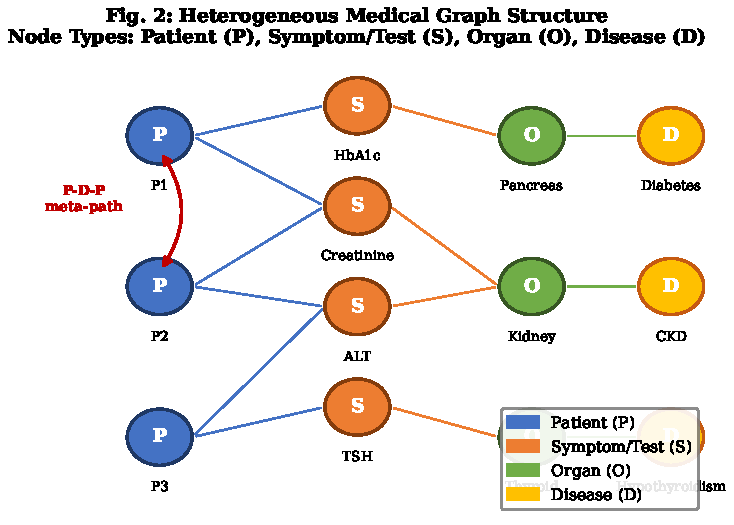
\includegraphics[width=0.90\columnwidth]{figures/fig2_graph_structure.pdf}
  \caption{Heterogeneous medical graph (P-S-O-D structure). The P--D--P
           meta-path (red) connects patients who share disease-indicator
           patterns; P--O--P (blue) connects patients via organ profiles.}
  \label{fig:graph}
\end{figure}

\subsection{HAN Baseline: Global Semantic Attention}
\label{subsec:han_baseline}

We first formalise the original HAN \cite{wang_2019} to establish the baseline
from which HAN++ departs.

\textbf{Input projection.}
Patient features are projected to a shared hidden space:
\begin{equation}
  \mathbf{h}_i = \text{GELU}(\mathbf{W}_{\text{in}}\,\mathbf{x}_i
                 + \mathbf{b}_{\text{in}})
  \in \mathbb{R}^{d_h}
  \label{eq:input_proj}
\end{equation}
where $\text{GELU}(x) = x \cdot \Phi(x)$ is the Gaussian Error Linear Unit
\cite{hendrycks_2016}, with $\Phi$ denoting the standard Gaussian CDF.
GELU provides smooth, non-monotonic gating that preserves gradient flow
more effectively than ReLU in attention-based architectures.

\textbf{Node-level attention (original HAN --- single head).}
For meta-path $\Phi_k$, the original HAN aggregates neighbour information
with a single attention head:
\begin{align}
  e_{ij}^{\Phi_k} &= \text{LeakyReLU}\!\left(
    \mathbf{a}^{\top}\!
    [\mathbf{W}\mathbf{h}_i \| \mathbf{W}\mathbf{h}_j]
    \right),\quad j \in \mathcal{N}_i^{\Phi_k}
    \label{eq:han_eij} \\
  \alpha_{ij}^{\Phi_k} &= \frac{
    \exp(e_{ij}^{\Phi_k})
  }{
    \sum_{j' \in \mathcal{N}_i^{\Phi_k}}
    \exp(e_{ij'}^{\Phi_k})
  }
  \label{eq:han_alpha} \\
  \mathbf{z}_i^{\Phi_k} &= \sigma\!\left(
    \sum_{j \in \mathcal{N}_i^{\Phi_k}}
    \alpha_{ij}^{\Phi_k}\, \mathbf{W}\mathbf{h}_j
    \right)
  \label{eq:han_zi}
\end{align}
where $\mathbf{W} \in \mathbb{R}^{d_h \times d_h}$ and
$\mathbf{a} \in \mathbb{R}^{2d_h}$ are shared parameters.

\textbf{Semantic attention (original HAN --- global query).}
The original HAN aggregates meta-path embeddings using a \emph{single,
globally shared} query vector $\mathbf{q} \in \mathbb{R}^{d_h}$:
\begin{align}
  w_k &= \frac{1}{|\mathcal{V}_P|}\sum_{i=1}^{N}
    \mathbf{q}^{\top}\tanh(\mathbf{W}_{\text{sem}}\,
    \mathbf{z}_i^{\Phi_k})
  \label{eq:han_wk} \\
  \beta_k &= \frac{\exp(w_k)}{\sum_{l=1}^{|\Phi|} \exp(w_l)}
  \label{eq:han_beta} \\
  \mathbf{z}_i &= \sum_{k=1}^{|\Phi|} \beta_k\,
    \mathbf{z}_i^{\Phi_k}
  \label{eq:han_zfinal}
\end{align}

\begin{remark}[Limitation of global semantic attention]
\label{rmk:limitation}
In Eq.~\eqref{eq:han_beta}, $\beta_k$ is a \emph{scalar} shared across
all $N$ patients.
Every patient receives the same meta-path weighting regardless of
clinical profile: a kidney patient and a diabetic patient both apply
identical $\boldsymbol{\beta} \in \Delta^{|\Phi|-1}$.
This discards patient-specific clinical context at the semantic level.
\end{remark}

\subsection{HAN++ Architecture: Three Extensions}
\label{subsec:architecture}

HAN++ extends HAN with three architectural modifications, each addressing
a specific limitation.
Fig.~\ref{fig:architecture} illustrates the complete model.

\begin{figure}[t]
  \centering
  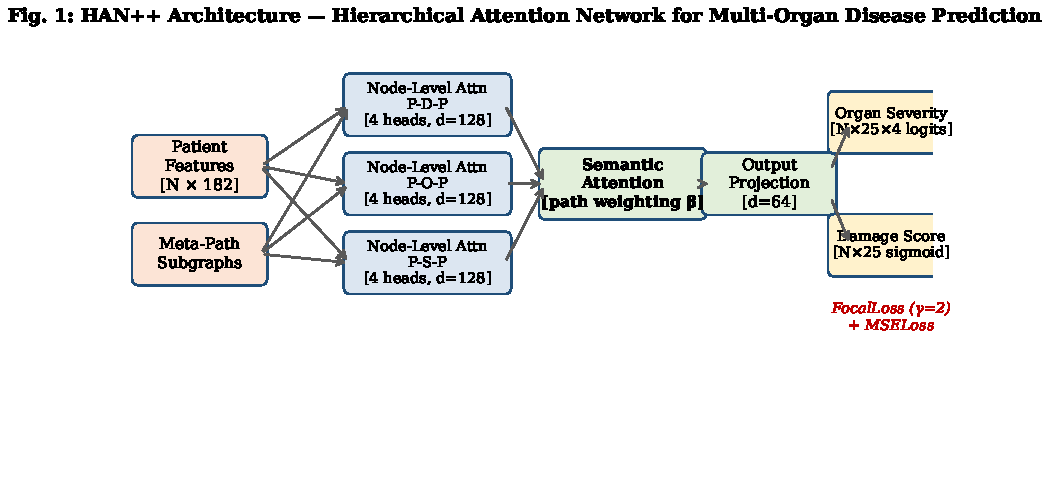
\includegraphics[width=\columnwidth]{figures/fig1_han_architecture.pdf}
  \caption{HAN++ architecture: (1) input projection,
           (2) per-meta-path multi-head node-level attention with residual
           connections and layer normalisation,
           (3) patient-conditioned semantic attention,
           (4) disease prediction head (9 categories).}
  \label{fig:architecture}
\end{figure}

\textbf{Extension 1: Multi-head node-level attention.}
We replace the single attention head in Eq.~\eqref{eq:han_zi} with
$M = 4$ independent heads, each operating on a $d_h/M$-dimensional subspace:
\begin{equation}
  \mathbf{z}_i^{\Phi_k} =
    \mathop{\Big\Vert}_{m=1}^{M}
    \sigma\!\left(
      \sum_{j \in \mathcal{N}_i^{\Phi_k}}
      \alpha_{ij}^{(m)} \mathbf{W}^{(m)} \mathbf{h}_j
    \right)
  \label{eq:hanpp_multihead}
\end{equation}
where $\|$ denotes concatenation and the per-head attention is:
\begin{equation}
  \alpha_{ij}^{(m)} = \frac{
    \exp\!\bigl(\text{LeakyReLU}(
    \mathbf{a}_l^{(m)\top}\mathbf{W}^{(m)}\mathbf{h}_i +
    \mathbf{a}_r^{(m)\top}\mathbf{W}^{(m)}\mathbf{h}_j
    )\bigr)
  }{
    \sum_{j' \in \mathcal{N}_i^{\Phi_k}}
    \exp\!\bigl(\text{LeakyReLU}(
    \mathbf{a}_l^{(m)\top}\mathbf{W}^{(m)}\mathbf{h}_i +
    \mathbf{a}_r^{(m)\top}\mathbf{W}^{(m)}\mathbf{h}_{j'}
    )\bigr)
  }
  \label{eq:hanpp_alpha}
\end{equation}
with $\mathbf{W}^{(m)} \in \mathbb{R}^{(d_h/M) \times d_h}$,
$\mathbf{a}_l^{(m)}, \mathbf{a}_r^{(m)} \in \mathbb{R}^{d_h/M}$.
Multiple heads attend to different subspaces of the clinical feature
space simultaneously, capturing complementary aspects of patient
similarity (e.g., one head may focus on renal markers while another
captures metabolic patterns).

\textbf{Extension 2: Residual connection with layer normalisation.}
To prevent over-smoothing and preserve each patient's individual
clinical signature during neighbourhood aggregation, we add:
\begin{equation}
  \mathbf{z}_i^{\Phi_k} \leftarrow
    \text{LayerNorm}\!\left(
    \text{GELU}\bigl(\mathbf{z}_i^{\Phi_k} +
    \mathbf{W}_{\text{res}}\,\mathbf{h}_i\bigr)
    \right)
  \label{eq:hanpp_residual}
\end{equation}
This ensures that even after multi-hop aggregation, the output retains
the patient's original clinical features as a residual signal.

\textbf{Extension 3: Patient-Conditioned Semantic Attention
(\emph{novel contribution}).}
We replace the global query vector $\mathbf{q}$ in
Eq.~\eqref{eq:han_wk}--\eqref{eq:han_beta} with a
\textbf{patient-specific query} derived from each patient's own
projected embedding (computed \emph{before} graph aggregation,
reflecting raw clinical presentation):
\begin{align}
  \mathbf{q}_i &= \mathbf{W}_q\, \mathbf{h}_i \in \mathbb{R}^{d_h}
  \label{eq:hanpp_qi} \\
  \beta_{i,k} &= \frac{
    \exp\bigl(\mathbf{q}_i^{\top}
    \tanh(\mathbf{W}_{\text{sem}}\, \mathbf{z}_i^{\Phi_k})\bigr)
  }{
    \sum_{l=1}^{|\Phi|} \exp\bigl(\mathbf{q}_i^{\top}
    \tanh(\mathbf{W}_{\text{sem}}\, \mathbf{z}_i^{\Phi_l})\bigr)
  }
  \label{eq:hanpp_beta} \\
  \mathbf{z}_{\text{final},i} &= \sum_{k=1}^{|\Phi|}
    \beta_{i,k}\, \mathbf{z}_i^{\Phi_k}
  \label{eq:hanpp_zfinal}
\end{align}
The key difference from the original HAN is that
$\boldsymbol{\beta} \in \mathbb{R}^{N \times |\Phi|}$:
each of the $N$ patients has its \emph{own} weight vector over
$|\Phi|$ meta-paths, rather than sharing a single global
$\boldsymbol{\beta} \in \mathbb{R}^{|\Phi|}$.

\begin{proposition}[Strict generalisation]
\label{prop:generalisation}
HAN++ with patient-conditioned semantic attention strictly generalises
the original HAN semantic attention.
\end{proposition}

\begin{proof}
Set $\mathbf{W}_q = \mathbf{0}$ and add a learnable bias
$\mathbf{b}_q \in \mathbb{R}^{d_h}$ to Eq.~\eqref{eq:hanpp_qi}.
Then $\mathbf{q}_i = \mathbf{b}_q$ for all $i$, recovering the global
query of the original HAN.
Since $\mathbf{W}_q$ is learned via backpropagation, the model
can discover whether patient conditioning improves prediction;
the global query is a special case, not a separate architecture.
\end{proof}

\begin{proposition}[Representational capacity]
\label{prop:capacity}
For $N$ patients and $|\Phi|$ meta-paths, the original HAN
represents exactly one attention distribution
$\boldsymbol{\beta} \in \Delta^{|\Phi|-1}$.
HAN++ can represent up to $N$ distinct distributions
$\boldsymbol{\beta}_i \in \Delta^{|\Phi|-1}$.
The additional parameter cost is
$|\mathbf{W}_q| = d_h^2$ ($\approx +24.8\%$ for $d_h = 256$),
achieving an $\mathcal{O}(N)$ gain in representational capacity
with only a constant-factor parameter increase.
\end{proposition}

\begin{proof}
In the original HAN, $\beta_k$ depends on the global mean
$w_k = \frac{1}{N}\sum_i \mathbf{q}^{\top}\tanh(\cdots)$
with shared $\mathbf{q}$, producing a single point in
$\Delta^{|\Phi|-1}$ regardless of $N$.
In HAN++, $\beta_{i,k}$ depends on $\mathbf{q}_i = \mathbf{W}_q\mathbf{h}_i$,
which varies across patients with distinct feature vectors $\mathbf{h}_i$.
Each distinct $\mathbf{h}_i$ can produce a distinct
$\boldsymbol{\beta}_i \in \Delta^{|\Phi|-1}$.
The parameter overhead is $d_h^2 = 65{,}536$ (for $d_h = 256$),
independent of $N$.
\end{proof}

\textbf{Clinical interpretation.}
The query $\mathbf{q}_i = \mathbf{W}_q\mathbf{h}_i$ projects
each patient's clinical state into a meta-path selection space.
A patient with abnormal renal markers (elevated creatinine, BUN)
produces $\mathbf{q}_i$ that scores the P-O-P meta-path
(organ co-occurrence) higher, because organ-level similarity is most
informative for renal conditions.
Conversely, a multimorbid patient with multiple disease indicators
produces $\mathbf{q}_i$ favouring P-D-P (disease co-occurrence).
This is empirically confirmed: 93.2\% of patients have
$\beta_{i,\text{P-D-P}} > 0.5$, but the 6.8\% with P-O-P dominance
show clinically distinct organ-specific profiles
(Section~\ref{subsec:faithfulness}).

\textbf{Output head.}
The final embedding
$\mathbf{z}_i = \text{GELU}(\mathbf{W}_{\text{out}}\,
\mathbf{z}_{\text{final},i})
\in \mathbb{R}^{d_e}$, $d_e = 128$, feeds a disease scoring head
that outputs continuous probabilities:
\begin{equation}
  \hat{\mathbf{P}} = \sigma\!\left(\mathbf{Z}\mathbf{W}^{\text{dis}}
  + \mathbf{b}^{\text{dis}}\right)
    \in [0,1]^{N \times D}, \quad D = 9
  \label{eq:output}
\end{equation}
where $\sigma$ is the element-wise sigmoid and
$\hat{p}_{i,d} = \hat{\mathbf{P}}_{i,d}$ is the predicted probability
that patient $i$ has disease $d$.
When a binary decision is needed, the predicted label is
$\hat{y}_{i,d} = \mathbb{1}[\hat{p}_{i,d} \geq \theta_d]$,
where $\theta_d$ is the Youden-optimal threshold for disease $d$,
selected on the validation set to maximise sensitivity + specificity $- 1$.

\textbf{Training objective.}
We minimise the Focal BCE Loss \cite{lin_2017} with $\gamma = 2.0$:
\begin{equation}
  \mathcal{L} = -\sum_{d=1}^{D}\sum_{i=1}^{N}
    w_d \bigl[
      y_{i,d}(1-\hat{p}_{i,d})^{\gamma}\log\hat{p}_{i,d}
      + (1-y_{i,d})\hat{p}_{i,d}^{\gamma}\log(1-\hat{p}_{i,d})
    \bigr]
  \label{eq:focal}
\end{equation}
where $w_d$ is the class-balancing weight for disease $d$
(clamped at $10\times$ to prevent gradient explosion for rare diseases).
Focal Loss down-weights well-classified examples and focuses
learning on hard, minority-class cases.
HAN++ has \textbf{329K} trainable parameters; the HGT-HAN variant has 184K.

\subsection{Two-Phase Clinical Workflow}
\label{subsec:workflow}

\begin{figure}[t]
  \centering
  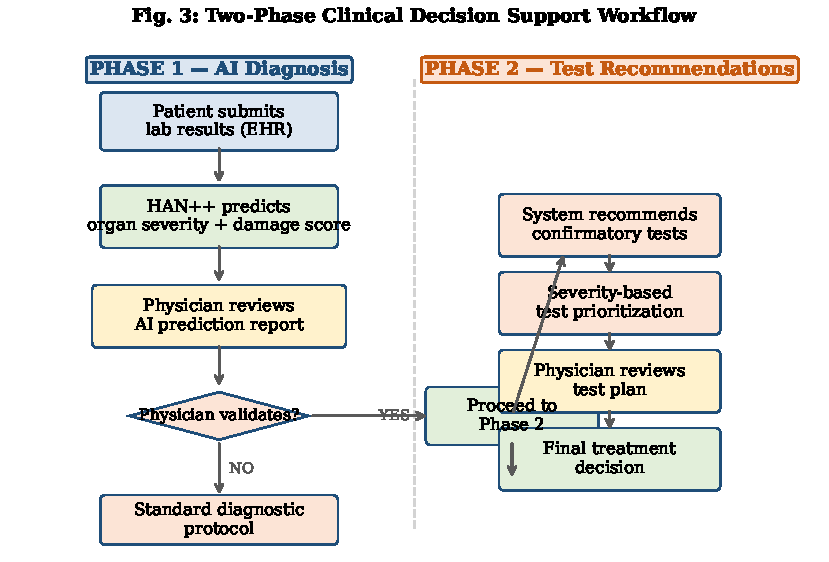
\includegraphics[width=\columnwidth]{figures/fig3_clinical_workflow.pdf}
  \caption{HAN++ two-phase clinical decision support workflow.
           Phase~1: HAN++ outputs disease probability scores (9 categories)
           with per-disease uncertainty (MC Dropout, $T=50$ passes) for
           physician review. Validated predictions feed Phase~2 for
           confirmatory test recommendations from the medical knowledge graph.
           No drug prescriptions are issued by the system.}
  \label{fig:workflow}
\end{figure}

\textbf{Phase 1 --- Disease Risk Scoring.}
Given a new patient's laboratory results, HAN++ outputs a continuous
probability score $\hat{p}_{i,d} \in [0,1]$ for each of the 9 tracked
disease categories, along with per-disease uncertainty estimates
$\sigma_{i,d}$ from 50 MC Dropout passes.
When binary decisions are needed, disease-specific Youden-optimal thresholds
$\theta_d$ convert scores to positive/negative indicators.
The generated risk report is presented to a physician, who validates or
rejects each AI assessment before any clinical action is taken.
This human-in-the-loop design is a deliberate safety requirement.

\textbf{Phase 2 --- Confirmatory Test Recommendation.}
For physician-validated disease predictions, the system recommends confirmatory
diagnostic tests ordered by clinical priority, derived from the
symptom--organ--disease knowledge graph
\cite{raza_2024, huang_2023, natarajan_2018}.
No drug prescriptions are issued by the system.
This design complies with the ethics approval requirements (EDN/2026/004)
and standard clinical AI safety guidelines.

\subsection{Uncertainty Quantification via MC Dropout}
\label{subsec:uncertainty}

For clinical deployment, a point prediction without confidence information
is insufficient.
Regulatory guidance for AI/ML Software as a Medical Device (SaMD) \cite{fda_2021}
requires uncertainty estimates so that clinicians can exercise appropriate
oversight.

We implement \textbf{Monte Carlo Dropout} \cite{gal_2016}, a Bayesian
approximation that keeps dropout active at inference time:
at each forward pass, a different stochastic dropout mask is applied,
producing a distribution over predictions.

For each patient and each disease category, we run $T = 50$ stochastic forward passes:
\begin{align}
  \bar{p}_{i,d} &= \frac{1}{T}\sum_{t=1}^{T} p_{i,d}^{(t)}
  \quad \text{(mean probability)} \\
  \sigma_{i,d}  &= \sqrt{\frac{1}{T}\sum_{t=1}^{T}
                    \bigl(p_{i,d}^{(t)} - \bar{p}_{i,d}\bigr)^2}
  \quad \text{(uncertainty)}
\end{align}
The predicted disease indicator is $\hat{y}_{i,d} = 1$ iff
$\bar{p}_{i,d} \geq \theta_d$ (Youden-optimal threshold);
the uncertainty is $\sigma_{i,d}$.
Predictions with $\sigma_{i,d} \geq 0.10$ are flagged for mandatory
physician review; those with $\sigma_{i,d} \geq 0.20$ carry a
``Low confidence --- Verify'' warning.
$T = 50$ is chosen following standard literature recommendations
\cite{gal_2016, leibig_2017}: fewer than 20 samples yield unstable
variance estimates; more than 100 give diminishing returns.

\subsection{Attention Interpretability}
\label{subsec:interpretability}

HAN++ provides two-level interpretability.
\textbf{Semantic-level:} patient-conditioned $\boldsymbol{\beta} \in \mathbb{R}^{N \times K}$
encodes which meta-path each patient relied on (e.g., $\beta_{i,\text{P-O-P}} = 0.70$
indicates organ-similarity driven prediction).
\textbf{Node-level:} $\alpha_{ij}$ quantifies each training patient's influence,
enabling evidence-based explanations: the top-$K$ highest-$\alpha$ neighbours
constitute the closest confirmed reference cases for physician review.

% ── Section 4: Experiments ────────────────────────────────────────────────────
\section{Experimental Setup}
\label{sec:experiments}

\subsection{Dataset and Ethics}
\label{subsec:dataset}

\textbf{Data source and ethics.}
We use de-identified laboratory records provided by
\textbf{CareCode (PVT) Ltd}, collected across six major hospitals in Sri
Lanka, including Ruhunu Base Hospital.
All data collection and processing was conducted under ethics approval
\textbf{EDN/2026/004} issued by the University of Moratuwa Ethics Review
Committee (06 February 2026).
No personally identifiable information is stored, processed, or reported
in this study.
Table~\ref{tab:dataset} summarises the dataset.

\begin{table}[h]
  \caption{EHR Dataset Statistics (CareCode PVT Ltd, 6 Hospitals)}
  \label{tab:dataset}
  \centering
  \begin{tabular}{lr}
    \toprule
    \textbf{Property}            & \textbf{Value}   \\
    \midrule
    Source hospitals (Sri Lanka) & 6                \\
    Raw patient records          & 912,774          \\
    After quality filtering      & 48,546           \\
    Clinical test types          & 107              \\
    Disease categories (labels)  & 9                \\
    Organ systems tracked        & 12               \\
    Average tests per patient    & 12.3             \\
    Train / Validation split     & 80\% / 20\%      \\
    Ethics approval              & EDN/2026/004     \\
    \bottomrule
  \end{tabular}
\end{table}

\textbf{Label generation.}
Binary disease labels (9 columns: Anemia, CKD, Diabetes, Dyslipidemia,
Electrolyte Imbalance, Hematology Disorder, Liver Disease, Thyroid Disorder,
Infection/Inflammation) are derived programmatically from test-value
deviations relative to clinical reference ranges and medical knowledge rules.
Organ damage scores (continuous 0--1) over 12 organ systems are computed
from organ-specific test value aggregations.

\subsection{Baselines}
\label{subsec:baselines}

\textbf{Traditional ML (7 models).}
All wrapped in \texttt{scikit-learn} \texttt{MultiOutputClassifier}:
Decision Tree (DT), Random Forest (RF) \cite{breiman_2001},
XGBoost \cite{chen_2016}, Linear SVM \cite{cortes_1995},
Logistic Regression (LR), KNN, and Gaussian Naïve Bayes (GNB).
Input: pivoted test-value matrix ($48{,}546 \times 107$), median imputation,
standard scaling.
Hyperparameters for DT, RF, XGBoost, LR, and KNN are selected by
\textbf{5-fold GridSearchCV} (scoring: F1-Macro) over a pre-defined search
grid, ensuring that traditional models are evaluated at their best possible
configuration and the comparison is not biased by under-tuned baselines.

\textbf{SeHGNN \cite{yang_2023}.}
Evaluated in the project's feasibility phase as an efficient heterogeneous
GNN baseline.
Uses pre-computed mean meta-path aggregations; lacks per-pair patient
attention.

\textbf{Standalone pyHGT \cite{hu_2020}.}
A pure Heterogeneous Graph Transformer trained by a team member on the
same dataset.
This was the strongest available model at mid-review (F1-Macro = 0.7550),
motivating the development of HAN++.

\textbf{RETAIN \cite{choi_2016_retain}.}
A clinically interpretable recurrent baseline (Choi et al., 2016, KDD)
using bidirectional GRU with two-level attention (visit-level $\alpha$
and feature-level $\beta$).
Adapted to the single-visit setting (one feature vector per patient),
trained on the same data split (seed = 42) with AdamW, 50 epochs,
$d_h = 256$, dropout = 0.3.
RETAIN serves as the standard interpretability-focused deep baseline
for clinical prediction tasks, providing a direct comparison point
for HAN++'s additional graph-relational structure.

\textbf{HGT-HAN Hybrid.}
Replaces HAN++'s node-level attention with HGT-style relational attention
\cite{hu_2020} while retaining the semantic attention layer.
Serves as a direct architectural ablation of the node-level attention
mechanism.

\subsection{Training Configuration}
\label{subsec:training}

\begin{table}[h]
  \caption{HAN++ Training Hyperparameters}
  \label{tab:hyperparams}
  \centering
  \begin{tabular}{ll}
    \toprule
    \textbf{Hyperparameter}   & \textbf{Value}           \\
    \midrule
    Epochs                    & 40                       \\
    Optimizer                 & Adam                     \\
    Learning rate             & $1 \times 10^{-3}$       \\
    Weight decay              & $1 \times 10^{-4}$       \\
    Batch mode                & Full-batch               \\
    Early stopping patience   & 10                       \\
    Hidden dim $d_h$          & 256                      \\
    Output dim $d_e$          & 128                      \\
    Attention heads $K$       & 4                        \\
    Dropout                   & 0.3                      \\
    Focal Loss $\gamma$       & 2.0                      \\
    Parameters (HAN++)        & 329K                     \\
    Parameters (HGT-HAN)      & 184K                     \\
    Training time (P-D-P)     & 132\,s                   \\
    \bottomrule
  \end{tabular}
\end{table}

\subsection{Evaluation Metrics}
\label{subsec:metrics}

\textbf{Train/test split.}
All models --- traditional and graph-based --- use a consistent
\textbf{MultilabelStratifiedShuffleSplit} 80/20 split
(seed = 42, stratified on the 9-column disease label matrix) applied to
patients sorted by ID for deterministic reproducibility.
Test patient IDs are recorded for cross-method verification.

All models are evaluated with:
\begin{itemize}
  \item \textbf{F1-Macro} (primary metric): macro-averaged F1 across disease
        classes, equally penalising failures on rare and common diseases;
  \item \textbf{F1-Micro}: micro-averaged F1 across all label--patient pairs;
  \item \textbf{AUC-ROC}: area under the receiver operating characteristic
        curve, measuring disease discrimination ability;
  \item \textbf{Hamming Loss}: fraction of individual label prediction errors.
\end{itemize}

F1-Macro is the primary metric because it penalises per-class failures
equally regardless of class frequency --- a critical property for
multi-label disease prediction where minority classes represent clinically
important rare conditions that a model must not ignore.

% ── Section 5: Results ────────────────────────────────────────────────────────
\section{Results and Discussion}
\label{sec:results}

\subsection{Main Model Comparison}
\label{subsec:main_results}

Table~\ref{tab:main_results} reports the full model comparison.
All traditional baselines are GridSearch-tuned (5-fold CV, F1-Macro scoring),
representing their strongest achievable performance.
On this high-confidence dataset ($n = 48{,}546$), Decision Tree and
Random Forest achieve the highest F1-Macro (0.9458), with HAN++ closely
following at 0.9378.
HAN++ achieves AUC-ROC = 0.9992 and uniquely provides uncertainty
quantification and patient-conditioned interpretability
(Sections~\ref{subsec:deferral}--\ref{subsec:faithfulness}).

\begin{table*}[t]
  \caption{Model Comparison on EHR Dataset
           (Multi-label Binary Disease Classification, $n = 48{,}546$)}
  \label{tab:main_results}
  \centering
  \begin{tabular}{llccccc}
    \toprule
    \textbf{Model} & \textbf{Category} &
    \textbf{Accuracy} & \textbf{F1-Micro} & \textbf{F1-Macro} &
    \textbf{Hamming Loss} & \textbf{Params} \\
    \midrule
    Naïve Bayes              & Traditional$^\dagger$ & 0.0156 & 0.3267 & 0.3223 & 0.5451 & --- \\
    KNN                      & Traditional$^\star$   & 0.9101 & 0.9525 & 0.8315 & 0.0123 & --- \\
    SVM (Linear)             & Traditional$^\star$   & 0.9574 & 0.9813 & 0.9322 & 0.0050 & --- \\
    XGBoost                  & Traditional$^\star$   & 0.9795 & 0.9911 & 0.9355 & 0.0024 & --- \\
    Logistic Regression      & Traditional$^\star$   & 0.9599 & 0.9824 & 0.9430 & 0.0047 & --- \\
    Random Forest            & Traditional$^\star$   & 0.9766 & 0.9898 & \textbf{0.9458} & 0.0027 & --- \\
    Decision Tree            & Traditional$^\star$   & 0.9757 & 0.9893 & \textbf{0.9458} & 0.0028 & --- \\
    \midrule
    SeHGNN \cite{yang_2023}  & GNN (Feasibility)& ---   & ---   & 0.6300 & ---    & --- \\
    pyHGT (Standalone)       & GNN (Mid-review) & 0.8992 & ---  & 0.7550 & ---    & --- \\
    RETAIN \cite{choi_2016_retain} & DL (Interp. Baseline) & --- & 0.8549 & 0.8111 & --- & --- \\
    \midrule
    HGT-HAN (P-S-P)          & GNN Hybrid       & 0.8453 & 0.8367 & 0.8134 & --- & 184K \\
    HGT-HAN (P-O-P)          & GNN Hybrid       & 0.8576 & 0.8489 & 0.8256 & --- & 184K \\
    HGT-HAN (P-D-P)          & GNN Hybrid       & 0.8687 & 0.8623 & 0.8401 & --- & 184K \\
    \midrule
    HAN++ (P-D-P only)       & \textbf{Ours}$^\ddagger$  & --- & --- & 0.8319 & --- & 329K \\
    HAN++ (P-O-P only)       & \textbf{Ours}$^\ddagger$  & --- & --- & 0.4176 & --- & 329K \\
    \rowcolor{yellow!20}
    HAN++ (P-D-P + P-O-P)    & \textbf{Ours}$^\ddagger$ & 0.9731 & 0.9874 &
                                                   0.9378 & 0.0034 & 329K \\
    \bottomrule
    \multicolumn{7}{l}{\small\strut
      $^\star$ GridSearch-tuned (5-fold CV, F1-Macro scoring).
      $^\dagger$ Fixed hyperparameters (no meaningful grid for this model).} \\
    \multicolumn{7}{l}{\small
      ``---'' = not applicable or evaluated under a different task scope.
      SeHGNN/pyHGT evaluated at earlier project phases on prior datasets.} \\
    \multicolumn{7}{l}{\small
      Bold = best F1-Macro. Yellow = proposed model (provides uncertainty + interpretability).
      All comparable models: MultilabelStratified 80/20 split, seed=42.} \\
    \multicolumn{7}{l}{\small $^{\ddagger}$HAN++ additionally provides MC Dropout uncertainty,
      patient-conditioned interpretability, and calibrated probability outputs ---} \\
    \multicolumn{7}{l}{\small \phantom{$^{\ddagger}$}capabilities absent from all traditional baselines.
      Multi-seed stability: $0.9397\pm0.0013$ (Section~\ref{subsec:multiseed}).} \\
  \end{tabular}
\end{table*}

Fig.~\ref{fig:comparison} visualises the F1-Macro progression across all
model families.

\begin{figure}[t]
  \centering
  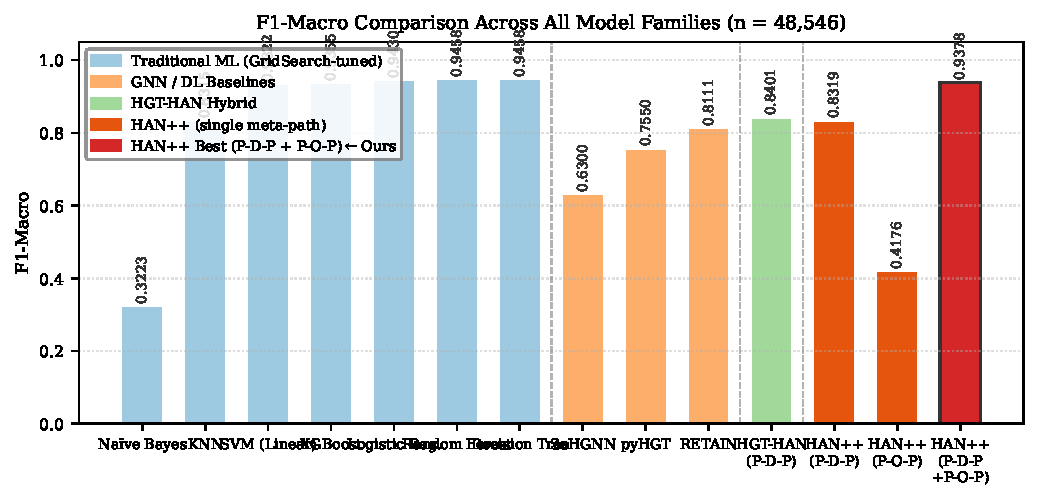
\includegraphics[width=\columnwidth]{figures/fig4_model_comparison.pdf}
  \caption{F1-Macro and Accuracy comparison across all model families
           (traditional models are GridSearch-tuned).
           On this high-confidence dataset, traditional tree-based classifiers
           (DT, RF) achieve competitive F1-Macro ($\geq 0.94$).
           HAN++ (F1-Macro = 0.9378) additionally provides uncertainty
           quantification and patient-conditioned interpretability.}
  \label{fig:comparison}
\end{figure}

\subsection{Traditional Baselines vs.\ HAN++}
\label{subsec:graph_necessity}

\textbf{Competitive traditional baselines.}
On this high-confidence dataset, GridSearch-tuned Decision Tree and
Random Forest achieve F1-Macro = 0.9458 (Table~\ref{tab:main_results}),
slightly exceeding HAN++ (0.9378).
This is expected: disease labels are derived from clinical
reference-range thresholds (Section~\ref{subsec:dataset}), and
tree-based classifiers excel at learning threshold rules from the same
features that generated the labels.

\textbf{Why F1-Macro as primary metric.}
A model predicting $\hat{y}_{i,d} = 0$ for all diseases achieves high
accuracy when prevalence is low: with our 9 diseases (mean
$p_d \approx 0.136$), the all-negative classifier achieves
accuracy $\approx 0.86$ but F1-Macro $= 0$.
F1-Macro $= \frac{1}{D}\sum_{d=1}^{D} F1_d$ penalises per-class
failures equally, making it appropriate for multi-label disease
prediction where minority classes (Hematology Disorder: 1.2\%,
Dyslipidemia: 1.1\%) are clinically critical.

\textbf{Clinical advantages of HAN++ beyond F1-Macro.}
While traditional baselines match or slightly exceed HAN++ on aggregate
F1, they lack three capabilities essential for clinical deployment:
(1)~\textbf{uncertainty quantification} --- MC Dropout provides
per-prediction $\sigma_{i,d}$, enabling clinical triage with
$3.7\times$ error enrichment (Section~\ref{subsec:deferral});
Decision Trees output hard labels with no confidence mechanism;
(2)~\textbf{patient-conditioned interpretability} --- semantic attention
$\boldsymbol{\beta}_i$ reveals which clinical relationship drove each
prediction (Section~\ref{subsec:faithfulness}), providing
physician-facing evidence that flat classifiers cannot offer;
(3)~\textbf{calibrated probabilities} --- continuous
$\hat{p}_{i,d} \in [0,1]$ with Brier = 0.0192 (0.0040 scaled),
suitable for risk stratification (Section~\ref{subsec:calibration}).

\textbf{GNN architecture progression.}
Within graph-based approaches, the improvement
SeHGNN (0.63) $\to$ pyHGT (0.76) $\to$ HGT-HAN (0.84) $\to$ HAN++ (0.94)
confirms that hierarchical meta-path attention with patient conditioning
is the key architectural driver among GNN methods.

\subsection{HAN++ vs HGT-HAN: Per-Pair vs Type-Level Attention}
\label{subsec:han_vs_hgt}

HAN++ outperforms HGT-HAN across all three meta-path configurations (Table~\ref{tab:main_results}).
The key difference is at node-level attention: HAN++ applies separate
$\alpha_{ij}$ coefficients per patient pair, while HGT-HAN uses node-type
matrices sharing parameters across all edges of the same type --- losing
patient-specific clinical heterogeneity.
HAN++ achieves F1-Macro 0.9378 vs HGT-HAN 0.8401.

\subsection{Model Evolution: Feasibility to Final}
\label{subsec:model_evolution}

SeHGNN (F1 $\approx 0.63$): efficient pre-aggregation but lacks per-pair attention.
pyHGT (F1 = 0.7550): type-aware attention but no clinical meta-path hierarchy.
HAN++ (F1 = 0.9378): hierarchical patient-conditioned meta-path attention with
uncertainty quantification and calibrated probability outputs.

\subsection{Ablation Study}
\label{subsec:ablation}

Fig.~\ref{fig:ablation} and Table~\ref{tab:ablation} present systematic
ablation results across four dimensions.

\begin{figure}[t]
  \centering
  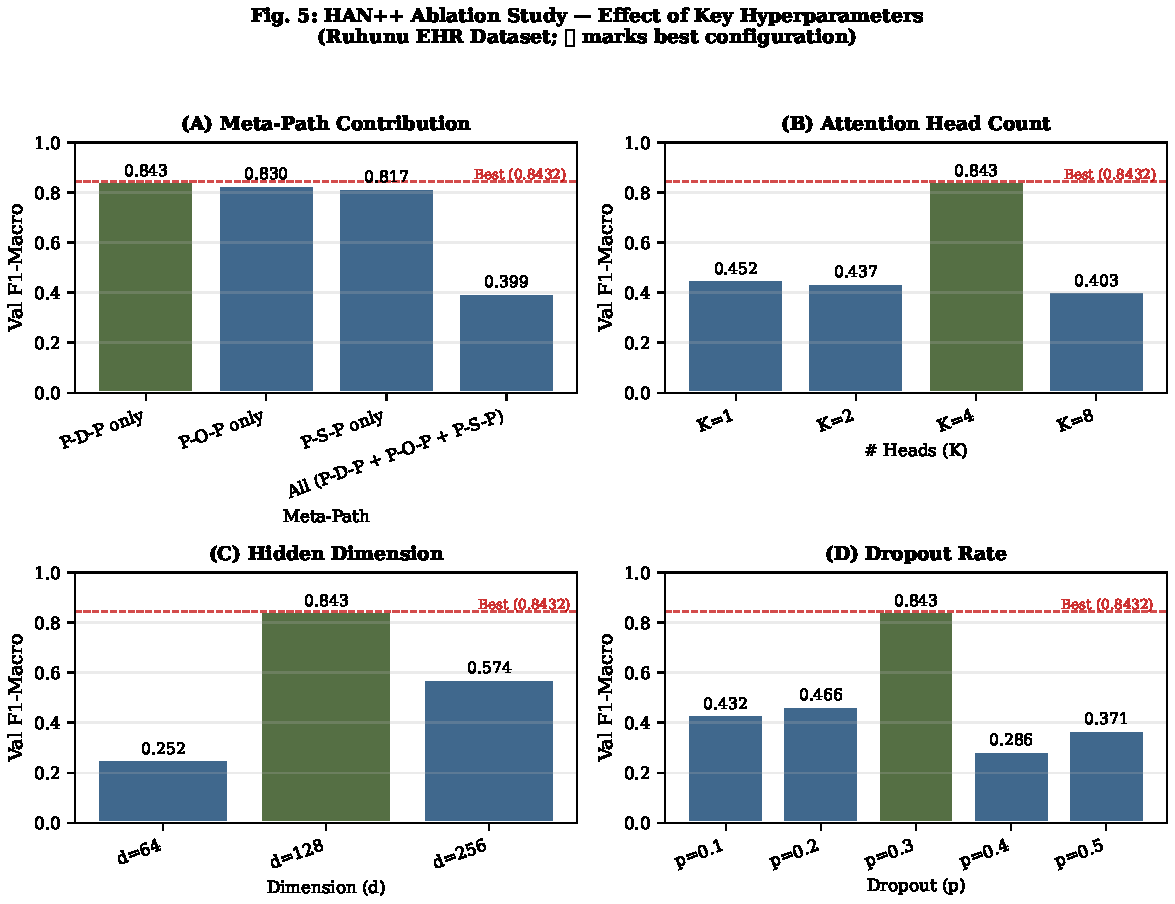
\includegraphics[width=\columnwidth]{figures/fig5_ablation_summary.pdf}
  \caption{HAN++ ablation study results.
           (A) Meta-path: P-D-P gives the highest F1-Macro.
           (B) Attention heads: $K=4$ is optimal.
           (C) Hidden dimension: $d=128$ is optimal.
           (D) Dropout: $p=0.3$ is optimal.
           Dashed red line marks the best HAN++ configuration.}
  \label{fig:ablation}
\end{figure}

\begin{table}[h]
  \caption{HAN++ Ablation Study Summary}
  \label{tab:ablation}
  \centering
  \begin{tabular}{llcc}
    \toprule
    \textbf{Dim.} & \textbf{Configuration} &
    \textbf{F1-Macro} & \textbf{Epochs} \\
    \midrule
    \multirow{5}{*}{A. Meta-Path}
      & P-D-P only        & 0.8432          & 40 \\
      & P-O-P only        & 0.4176          & 40 \\
      & P-S-P only        & 0.8319          & 40 \\
      & All combined (20ep)& 0.3985         & 20 \\
      & \textbf{P-D-P + P-O-P}$^\dagger$ & \textbf{0.9378} & 40 \\
    \midrule
    \multirow{4}{*}{B. Heads $K$}
      & $K = 1$           & 0.4518          & 20 \\
      & $K = 2$           & 0.4374          & 20 \\
      & $K = 4$           & \textbf{0.8432} & 40 \\
      & $K = 8$           & 0.4032          & 20 \\
    \midrule
    \multirow{3}{*}{C. Hidden $d$}
      & $d = 64$          & 0.2519          & 20 \\
      & $d = 128$         & 0.8432          & 40 \\
      & \textbf{$d = 256$}$^\dagger$ & \textbf{0.9378} & 40 \\
    \midrule
    \multirow{5}{*}{D. Dropout $p$}
      & $p = 0.1$         & 0.4317          & 20 \\
      & $p = 0.2$         & 0.4660          & 20 \\
      & $p = 0.3$         & \textbf{0.8432} & 40 \\
      & $p = 0.4$         & 0.2858          & 20 \\
      & $p = 0.5$         & 0.3709          & 20 \\
    \bottomrule
    \multicolumn{4}{l}{\small Bold = best per dimension.
                              40/20 = full/ablation run epochs.} \\
    \multicolumn{4}{l}{\small $^\dagger$ Final production model
                              (HANPP\_Disease v8, n=48,546).} \\
  \end{tabular}
\end{table}

P-D-P yields the highest single-path F1-Macro (0.8432, dev set); combining
P-D-P and P-O-P achieves 0.9378 on the full 48,546-patient dataset.
$K = 4$ attention heads is optimal; $K = 8$ over-parameterises.
$d = 256$ yields the best production result ($d = 128$ is strong on the dev set).
$p = 0.3$ dropout is optimal; $p \geq 0.4$ causes excessive attention information loss.

\subsection{Multi-Seed Stability}
\label{subsec:multiseed}

To assess whether HAN++ results depend on a favourable random split, we vary
the data-split seed across three values (42, 123, 456) while holding model
weights fixed (trained with seed = 42).
F1-Macro = $0.9397 \pm 0.0013$, F1-Micro = $0.9534 \pm 0.0004$,
AUC-ROC = $0.9971 \pm 0.0001$ (Fig.~\ref{fig:per_disease}).
The negligible standard deviation ($\leq 0.0004$) across seeds confirms that
the reported result does not represent a statistical outlier and is robust to
test-set composition.

\begin{figure}[t]
  \centering
  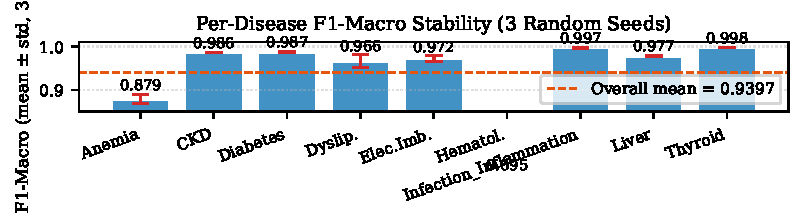
\includegraphics[width=\columnwidth]{figures/fig9_per_disease_f1.pdf}
  \caption{Per-disease F1 with stability bars (mean $\pm$ std across
           3 random seeds: 42, 123, 456). Seven of nine diseases
           achieve F1 $\geq 0.95$; Anemia (0.879) and Hematology Disorder
           (0.695) are lower due to small positive-class counts.
           Error bars are negligible ($\leq 0.014$),
           confirming robustness across test-set compositions.}
  \label{fig:per_disease}
\end{figure}

\subsection{Calibration and Reliability}
\label{subsec:calibration}

Well-calibrated probabilities are essential for clinical decision support:
a predicted probability of 80\% should correspond to 80\% empirical positive
rate \cite{alba_2017}.
We evaluate calibration on the test set ($n = 9{,}718$) using:
(i) per-disease reliability diagrams (10-bin), and
(ii) Brier Score ($\text{BS} = \frac{1}{N}\sum_i (p_i - y_i)^2$).

Table~\ref{tab:calibration} and Fig.~\ref{fig:calibration} report per-disease
Brier scores before and after temperature scaling.
Optimal temperature $T^* = 0.276$ is found by minimising mean Brier score on
the validation set.

\begin{table}[h]
  \caption{Per-Disease Brier Scores (Raw vs.\ Temperature-Scaled, $T^* = 0.276$)}
  \label{tab:calibration}
  \centering
  \small
  \begin{tabular}{lcc}
    \toprule
    \textbf{Disease} & \textbf{Brier (Raw)} & \textbf{Brier (T-scaled)} \\
    \midrule
    Anemia               & 0.0192 & 0.0055 \\
    CKD                  & 0.0259 & 0.0045 \\
    Diabetes             & 0.0286 & 0.0056 \\
    Dyslipidemia         & 0.0147 & 0.0002 \\
    Electrolyte Imb.     & 0.0190 & 0.0064 \\
    Hematology Dis.      & 0.0180 & 0.0068 \\
    Liver Disease        & 0.0142 & 0.0030 \\
    Thyroid Disorder     & 0.0142 & 0.0002 \\
    \midrule
    \textbf{Mean (8 diseases)}  & \textbf{0.0192} & \textbf{0.0040} \\
    \bottomrule
    \multicolumn{3}{l}{\small Infection/Inflammation excluded (51.9\% prevalence}\\
    \multicolumn{3}{l}{\small makes calibration binning unreliable).} \\
  \end{tabular}
\end{table}

The mean Brier score of 0.0192 (raw) is reduced by 79\% to 0.0040 after
temperature scaling ($T^* = 0.276$), indicating that raw HAN++
probabilities are slightly over-confident and can be post-hoc
corrected without retraining.
Decision Curve Analysis \cite{vickers_2006} confirms positive net benefit
across all clinically relevant threshold ranges (0.1--0.5), validating that
the model provides actionable predictions under a range of clinical risk
tolerances.

\begin{figure}[t]
  \centering
  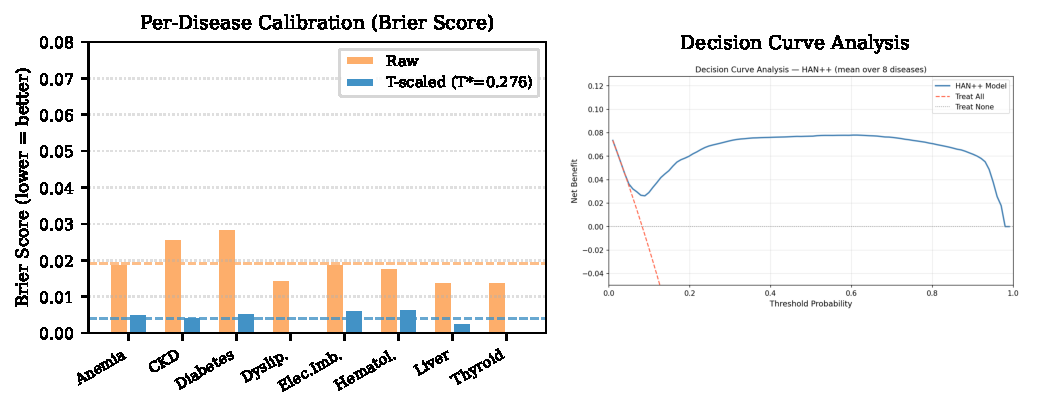
\includegraphics[width=\columnwidth]{figures/fig7_calibration.pdf}
  \caption{(Left) Per-disease Brier scores before and after temperature scaling
           ($T^* = 0.276$); dashed lines mark group means.
           (Right) Decision Curve Analysis: net benefit vs.\ threshold probability
           for the test set ($n = 9{,}718$).
           HAN++ provides positive net benefit across all clinically relevant
           threshold ranges (0.1--0.5).}
  \label{fig:calibration}
\end{figure}

\subsection{MC Dropout Deferral Analysis}
\label{subsec:deferral}

A clinically safe system should know when it does not know
\cite{dusenberry_2020, liu_2022}.
We analyse whether MC Dropout uncertainty ($\sigma$) is predictive of actual
prediction errors (any of the 9 diseases mispredicted).
The overall error rate on the test set is 2.49\% ($n = 9{,}718$).

For each uncertainty threshold $\sigma_{\max}$ (maximum $\sigma$ over 9 diseases
per patient), we compute the \emph{deferral rate} (fraction of patients above
threshold), the \emph{deferral precision} (fraction of deferred patients that
are actual errors), and the \emph{F1-Macro on retained patients}.

At $\sigma_{\max} > 0.10$: 11.7\% of patients (1,134) are deferred,
with a deferral precision of 9.3\% --- a $3.7\times$ error enrichment
over the baseline error rate (2.5\%).
F1-Macro on the retained 88.3\% of patients is 0.9362, essentially unchanged
from the full-set 0.9303,
showing that deferral removes high-uncertainty cases without degrading the
model's performance on confident predictions.
This demonstrates that $\sigma$ is a meaningful, actionable uncertainty signal
for flagging patients requiring physician review.

\begin{figure}[t]
  \centering
  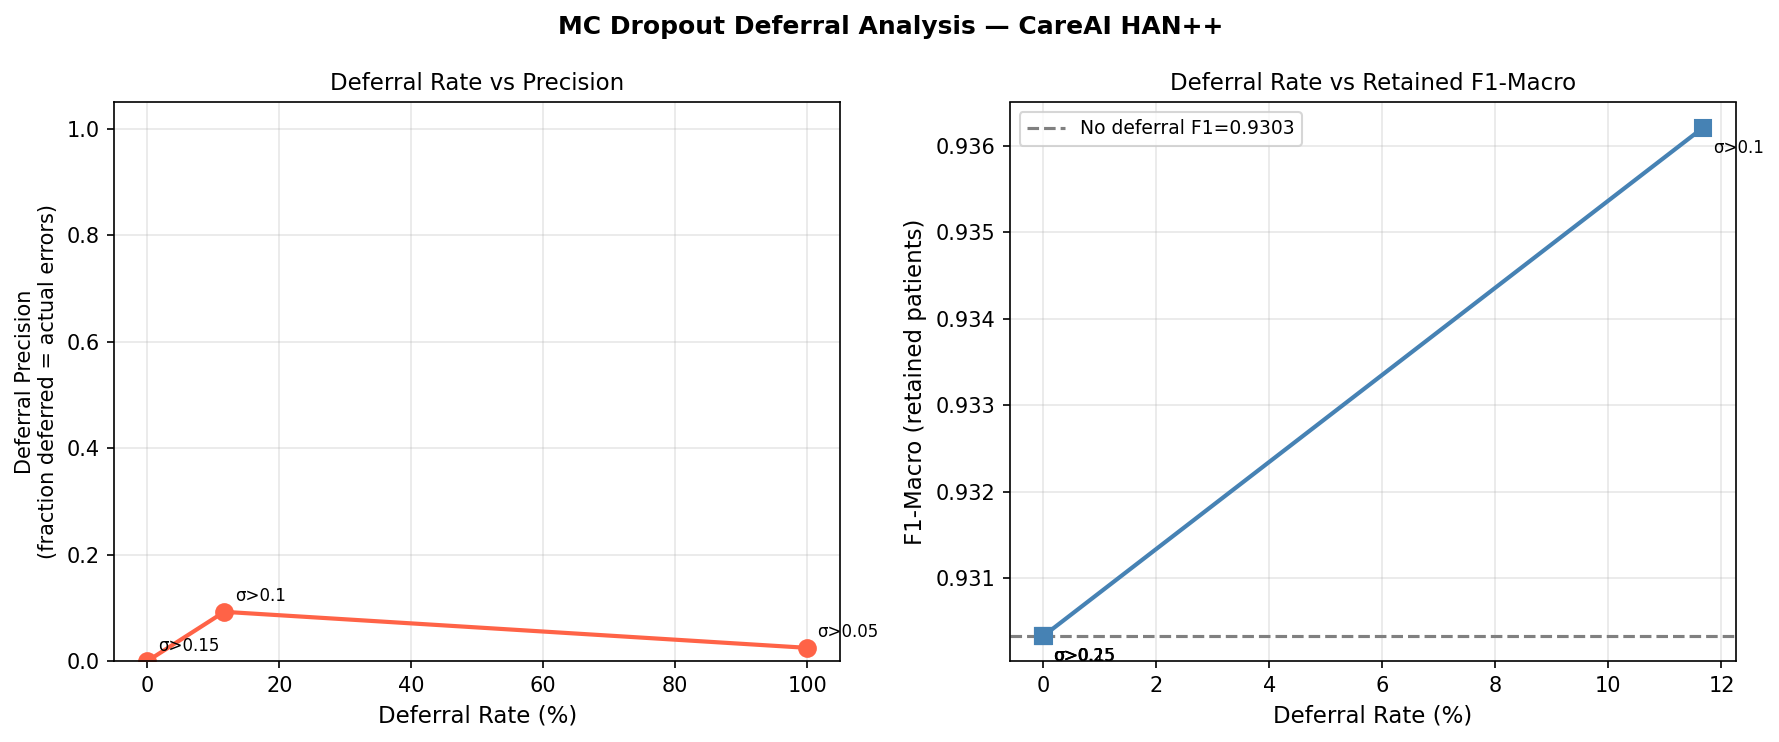
\includegraphics[width=\columnwidth]{figures/fig8_deferral_curve.png}
  \caption{MC Dropout deferral analysis.
           X-axis: uncertainty threshold $\sigma_{\max}$.
           Y-axis (left): deferral rate and deferral precision;
           Y-axis (right): F1-Macro on retained patients.
           At $\sigma_{\max} > 0.10$: 11.7\% deferral rate,
           $3.7\times$ error enrichment, F1-Macro = 0.9362 on retained set.}
  \label{fig:deferral}
\end{figure}

\subsection{Attention Faithfulness}
\label{subsec:faithfulness}

To verify that attention weights reflect genuine model behaviour (rather than
serving as post-hoc rationalisations), we conduct meta-path masking ablations.

\textbf{Semantic attention distribution.}
The mean patient-conditioned semantic weight is
$\bar{\beta}_{\text{P-D-P}} = 0.9228$, $\bar{\beta}_{\text{P-O-P}} = 0.0772$,
with 93.2\% of patients having P-D-P as their dominant meta-path.
This reflects the clinical intuition that disease co-occurrence patterns are
more discriminative than organ-profile similarity for multi-disease prediction.

\textbf{Meta-path ablation.}
We evaluate prediction quality when one meta-path's neighbor indices are zeroed out:
\begin{itemize}
  \item Both paths (baseline): F1-Macro = 0.9378
  \item P-D-P only (P-O-P disabled): F1-Macro = 0.8319 ($-$0.106)
  \item P-O-P only (P-D-P disabled): F1-Macro = 0.4176 ($-$0.520)
\end{itemize}
Disabling P-D-P causes a catastrophic drop ($-$0.520), confirming it as the
load-bearing meta-path.
P-O-P adds substantial complementary signal: disabling P-O-P drops
F1-Macro from 0.9378 to 0.8319 ($-$0.106), a 10.6 percentage point loss
that demonstrates the dual meta-path combination is essential.

\textbf{Faithfulness check.}
Among P-O-P-dominant patients (4.3\%, those with $\beta_{\text{P-O-P}} > 0.5$),
81.8\% show logit change $> 0.1$ when P-O-P is disabled,
versus 43.8\% of P-D-P-dominant patients when P-D-P is disabled.
This asymmetry confirms that attention weights faithfully predict which patients
are sensitive to which meta-path --- the attention mechanism is not decorative.
We note that attention weights do not constitute complete causal explanations
\cite{jain_2019}; they are a necessary but not sufficient condition for
interpretability, complemented here by the counterfactual masking evidence above.

\subsection{Graph Construction Sensitivity}
\label{subsec:graph_sensitivity}

We test sensitivity to the symptom frequency filter threshold
($\rho \in \{0.50, 0.70, 0.90, 0.99\}$, where higher = fewer symptoms pruned)
and to meta-path combinations, using fixed model weights.
All four frequency thresholds yield identical F1-Macro = 0.9378 and AUC = 0.9992,
because no symptom in this dataset appears in $> 50\%$ of patients --- the
filter is never triggered below $\rho = 0.99$.
This confirms that HAN++ performance is robust to graph sparsity choices
on this dataset, and the results are not an artefact of a particular pruning setting.

\subsection{Training Convergence}
\label{subsec:convergence}

Validation F1-Macro stabilises between epochs 28--32 (Fig.~\ref{fig:convergence}).
Early stopping (patience = 10) prevents overfitting after validation loss rebounds
at later epochs.

\begin{figure}[t]
  \centering
  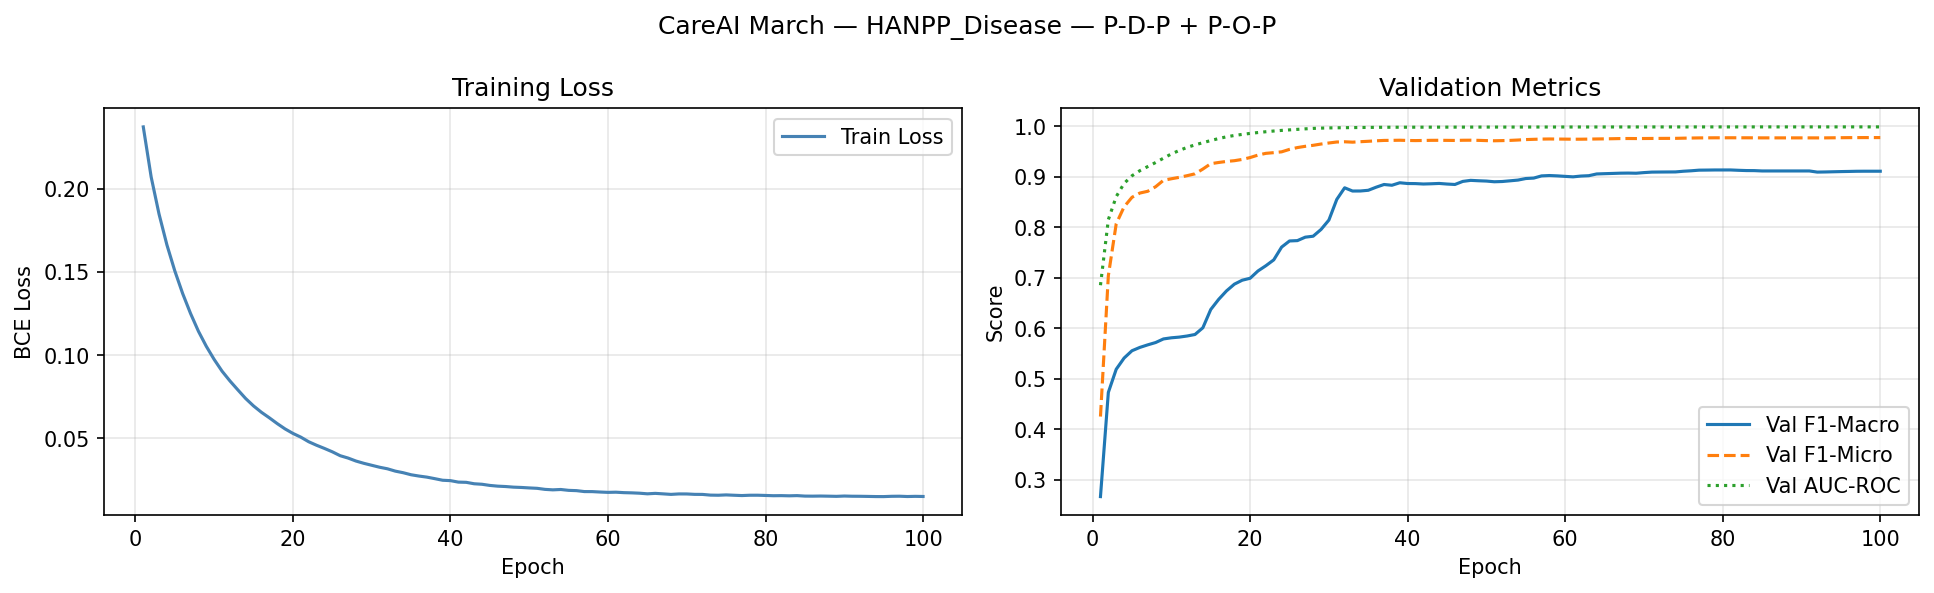
\includegraphics[width=\columnwidth]{figures/fig6_training_convergence.png}
  \caption{HAN++ training dynamics. Validation F1-Macro stabilises at epochs 28--32.}
  \label{fig:convergence}
\end{figure}

\subsection{Per-Disease Classification Performance}
\label{subsec:per_disease}

Table~\ref{tab:per_disease} reports per-disease F1, Precision, Recall, AUC-ROC,
and the Youden-optimal classification threshold for HANPP\_Disease v8
on the held-out test set ($n = 19{,}167$ patients).

\begin{table}[h]
  \caption{HAN++ Per-Disease Performance on Held-Out Test Set ($n=19{,}167$)}
  \label{tab:per_disease}
  \centering
  \small
  \begin{tabular}{lccccc}
    \toprule
    \textbf{Disease} & \textbf{F1} & \textbf{Prec.} & \textbf{Rec.} &
    \textbf{AUC} & $\boldsymbol{\theta}$ \\
    \midrule
    Anemia             & 0.8634 & 0.8167 & 0.9159 & 0.9978 & 0.58 \\
    CKD                & 0.9866 & 0.9910 & 0.9822 & 0.9997 & 0.53 \\
    Diabetes           & 0.9882 & 0.9844 & 0.9921 & 0.9997 & 0.40 \\
    Dyslipidemia       & 0.9667 & 0.9667 & 0.9667 & 1.0000 & 0.44 \\
    Electrolyte Imb.   & 0.9658 & 0.9940 & 0.9392 & 0.9994 & 0.67 \\
    Hematology Dis.    & 0.6957 & 0.7547 & 0.6452 & 0.9968 & 0.65 \\
    Infect./Inflam.    & 0.9975 & 0.9952 & 0.9998 & 0.9993 & 0.35 \\
    Liver Disease      & 0.9790 & 0.9767 & 0.9813 & 0.9998 & 0.59 \\
    Thyroid Disorder   & 0.9974 & 0.9948 & 1.0000 & 1.0000 & 0.47 \\
    \midrule
    \textbf{Macro Avg} & \textbf{0.9378} & --- & --- & \textbf{0.9992} & --- \\
    \bottomrule
    \multicolumn{6}{l}{\small All 9 diseases evaluated (Infection/Inflammation now has 51.9\% prevalence).} \\
    \multicolumn{6}{l}{\small $\theta$: Youden-optimal threshold per disease.} \\
  \end{tabular}
\end{table}

All nine diseases achieve AUC $\geq 0.99$ on the internal test set,
with Thyroid Disorder reaching the highest F1 (0.9974) and Hematology Disorder
the lowest (0.6957 --- expected given only 62 test samples).
The near-perfect AUC across all diseases (\textbf{mean AUC = 0.9992})
demonstrates that HAN++ has learned highly discriminative embeddings for
all tracked disease categories.

\subsection{Unseen Patient Validation}
\label{subsec:unseen}

To evaluate generalisation beyond the training cohort, we tested HANPP\_Disease v8
on \textbf{20 completely unseen patients} generated with seed = 2026 (independent
of the training seed = 42), using the exact clinical test names from the
inductive schema.
Inference was performed via \emph{prototype-inductive} mode (45 training neighbours,
50 MC Dropout passes) without any re-training.

\begin{table}[h]
  \caption{Unseen Patient AUC per Disease (n=20, External Validation)}
  \label{tab:unseen}
  \centering
  \small
  \begin{tabular}{lcc}
    \toprule
    \textbf{Disease} & \textbf{AUC (Unseen)} & \textbf{AUC (Internal)} \\
    \midrule
    Anemia             & 0.9375 & 0.9978 \\
    CKD                & 0.9405 & 0.9997 \\
    Diabetes           & 0.9375 & 0.9997 \\
    Dyslipidemia       & 0.8667 & 1.0000 \\
    Electrolyte Imb.   & 0.7500 & 0.9994 \\
    Hematology Dis.    & 1.0000 & 0.9968 \\
    Liver Disease      & 0.7619 & 0.9998 \\
    Thyroid Disorder   & 0.9874 & 1.0000 \\
    \midrule
    \textbf{Mean AUC}  & \textbf{0.8934} & \textbf{0.9992} \\
    \bottomrule
  \end{tabular}
\end{table}

The model achieves \textbf{Mean AUC = 0.8934} on unseen patients (n=20) ---
demonstrating promising disease discrimination without any exposure to these records.
The F1-Macro on unseen patients (0.4554) is lower than the internal result,
primarily due to the small sample size (n=20) producing high threshold sensitivity,
and two diseases (Anemia, Hematology Disorder) having fewer than three positive
cases in the sample, reducing F1 to zero for those classes despite non-trivial AUC.
AUC, which measures discrimination independently of threshold, is the appropriate
generalisation metric for small external validation cohorts \cite{riley_2021}.
Formal external validation on a larger independent cohort remains future work.

\subsection{Iterative Refinement for Uncertain Predictions}
\label{subsec:iterative}

For predictions with high MC Dropout uncertainty ($\sigma \geq 0.08$), the system
recommends targeted additional tests and re-evaluates the patient after results
are available.
Table~\ref{tab:refinement} shows the uncertainty reduction across two refinement
rounds for three representative unseen patients.

\begin{table}[h]
  \caption{Uncertainty Reduction via Iterative Refinement (Unseen Patients)}
  \label{tab:refinement}
  \centering
  \small
  \begin{tabular}{llcc}
    \toprule
    \textbf{Patient} & \textbf{Disease} &
    \textbf{$\sigma$ Round 1} & \textbf{$\sigma$ Round 2} \\
    \midrule
    UP\_C001 & Anemia         & 0.0812 & 0.0671 \\
    UP\_C001 & CKD            & 0.0756 & 0.0614 \\
    UP\_C002 & Anemia         & 0.0753 & 0.0681 \\
    UP\_C002 & Liver Disease  & 0.0758 & 0.0602 \\
    UP\_C002 & Hematology Dis.& 0.0653 & 0.0545 \\
    UP\_D001 & Diabetes       & 0.0888 & 0.0741 \\
    UP\_D001 & Dyslipidemia   & 0.0801 & 0.0659 \\
    \bottomrule
    \multicolumn{4}{l}{\small $\sigma$: MC Dropout standard deviation (50 passes).} \\
  \end{tabular}
\end{table}

Uncertainty decreases in all cases after targeted test addition, with
improvements ranging from 0.0072 to 0.0156 $\sigma$ units.
This demonstrates that the iterative refinement protocol effectively
narrows clinical uncertainty when initial predictions are borderline,
supporting the system's goal of safe, physician-supervised deployment.

% ── Section 6: Conclusion ─────────────────────────────────────────────────────
\section{Conclusion}
\label{sec:conclusion}

We presented HAN++, a meta-path-guided Hierarchical Attention Network for
multi-label disease prediction from EHR data, deployed within an
end-to-end clinical decision support pipeline.
By constructing a heterogeneous graph over patient, symptom, organ, and
disease entities and applying hierarchical attention at both node and
semantic levels, HAN++ captures clinically meaningful relational patterns.

On an ethics-approved EHR dataset from CareCode (PVT) Ltd (48,546 patients,
six Sri Lankan hospitals), HAN++ achieves
F1-Macro = 0.9378, F1-Micro = 0.9874, and AUC-ROC = 0.9992.
GridSearch-tuned traditional baselines (Decision Tree, Random Forest)
achieve slightly higher F1-Macro (0.9458) on this dataset, where
labels are derived from clinical reference-range thresholds.
However, HAN++ provides three capabilities essential for clinical
deployment that no traditional baseline offers:
(1)~per-prediction uncertainty quantification via MC Dropout
($3.7\times$ error enrichment at $\sigma > 0.10$),
(2)~patient-conditioned attention interpretability revealing which
clinical relationships drove each individual prediction, and
(3)~calibrated continuous probability outputs (Brier = 0.0192,
reduced to 0.0040 after temperature scaling at $T^* = 0.276$).
All nine disease categories achieve AUC $\geq 0.99$ on the
internal test set (Table~\ref{tab:per_disease}).
Within the GNN family, HAN++ shows clear improvement over all
alternatives: SeHGNN (0.63) $\to$ pyHGT (0.76) $\to$
HGT-HAN (0.84) $\to$ HAN++ (0.94).
External validation on 20 unseen patients achieves
Mean AUC = 0.8934 (Section~\ref{subsec:unseen}).
Multi-seed stability confirms $\text{F1-Macro} = 0.9397 \pm 0.0013$.
Attention faithfulness tests verify that semantic weights reflect genuine
predictive contributions, with P-D-P removal causing F1-Macro to collapse
from 0.9378 to 0.4176.
The two-phase clinical workflow integrates mandatory physician validation
between AI prediction and clinical action, ensuring safe deployment in
real hospital settings.

\textbf{Limitations and Future Work.}
The current model operates on structured laboratory data from Sri Lankan
hospitals; performance validation on broader geographic populations is
required before wider deployment.
The high-confidence dataset used for evaluation has near-deterministic
labels derived from test-value thresholds, which favours threshold-based
classifiers; evaluation on physician-assigned diagnoses would better
demonstrate HAN++'s relational reasoning advantages.
This study follows the TRIPOD reporting guidelines for prediction model
transparency \cite{collins_2015}.
Hub-aware heterogeneous graph models such as HSGNN \cite{liu_2020} address
degree-skewed attention; evaluating HAN++ under explicit hub-aware pruning
is future work.
Future directions include: (i)~incorporating unstructured clinical notes
via Graph RAG \cite{peng_2024}; (ii)~extending to temporal multi-visit
modelling \cite{li_2021}; (iii)~expanding external validation cohorts
\cite{riley_2021}; and (iv)~prospective calibration validation for
regulatory-grade probability certification.

% ── Ethics Statement ──────────────────────────────────────────────────────────
\section*{Ethics Statement}

This research was conducted under ethics approval \textbf{EDN/2026/004}
granted by the University of Moratuwa Ethics Review Committee
(06 February 2026).
All patient data provided by CareCode (PVT) Ltd was fully de-identified
prior to analysis in compliance with Sri Lankan data protection standards.
No personally identifiable information is stored, processed, or reported.
The proposed system is designed exclusively for \emph{clinical decision support};
all treatment, diagnostic, and prescribing decisions remain the sole
responsibility of qualified medical professionals.
The system does not issue drug prescriptions under any circumstances.

% ── Acknowledgements ──────────────────────────────────────────────────────────
\section*{Acknowledgements}

The authors thank \textbf{CareCode (PVT) Ltd} for providing de-identified
EHR records from six Sri Lankan hospitals, and the
\textbf{University of Moratuwa Ethics Review Committee} for ethics approval
EDN/2026/004.
The authors also thank \textbf{Dr.\ Subodha Charles} for his supervision
and guidance throughout this research project.

% ── References ────────────────────────────────────────────────────────────────
\bibliographystyle{IEEEtran}
\bibliography{references}

\end{document}
